 Couchbase Server is designed to be an operational data store for real-time data access. It is a NoSQL database that facilitates both as a key-value and  document store database. A key-value able to store  any type of data including  strings, numbers and binary data and the data is generally treated as an opaque Binary Large Object(BLOB) that do not try to parse it at the time of query. For document store, data is stored in a valid JSON format. Couhbase Server stores data in logical unit called Buckets. Buckets are isolated to each other that have their own RAM quota and replica settings. These buckets can be compared as \texttt{database} in Mongodb or other RDBMS. Couchbase recommends few numbers of buckets in a single cluster. A Bucket  contains any type of data but data except JSON type can be retrieved only by their key. Therefore, it is important to check meta type of data that are stored in a single document before fetching. Each document is stored independently and there is not concept of grouping documents like collections in MongoDB or tables in other RDBMS. The document is separated by user-defined document type. 
\label{cb-metadata}
\paragraph{Metadata}
For every value stored in a bucket, Couchbase Server generates following meta information that is associated with a document~\cite[p. 26]{cb/ostrovsky2014pro}. 
\begin{itemize}
	\item{Expiration}
		The Time to Live(TTL) also named as expiration time is the life time of the document. The default value of TTL is 0 that indicates document will never expire and also can be set as Unix epoch time after which document is removed.
	
	\item{Check-and-Set(CAS)}
		The CAS value is 64-bit integer that is updated by server when associated item is modified. It enables to update information only if unique identifier matches the identifier of the document that needed to be updated. CAS is used to manage concurrency when multiple client attempts to update the same document simultaneously. 
	\item{Flags} are 32 bit integer and are set of SDK specific use. For example, format in which data is serialize or data type of the object being stored. \todo{what is this??? correct when in ROOM}
\end{itemize}	
In addition of TTL, CAS and flags, three other meta information are stored at the time of document creation. The document's key \textit{id} is saved as part of metadata, \textit{type} is the type of a document either \textit{json} or Base64 encoded string for all other.
\paragraph{Document key}
Every value in Couchbase Server is saved in unique key called document key. Unlike MongoDB, Couchbase  do not generate document key automatically and 250 characters string should be manually generated.
%In case of XMark data each \texttt{id} attributes of  \texttt{item}, \texttt{person}, \texttt{open\_auction}, \texttt{category} represent as key. In case of  \texttt{closed\_auction} and  \texttt{edge} key can be manually generated. 

\paragraph{Bucket and vBucket}
Couchbase Server uses data bucket as a logical container of information that provides a logical grouping of physical resources within a cluster~\citep{lichtenberg2013nosql}. Documents in Couchbase do not have their fixed schema and multiple documents  with different schema can be stored in same bucket. One or more attributes in documents are added to differentiate the various objects stored in a bucket and create indexes on them. Each bucket is split into 1024 logical partition called vBuckets. A vBucket is treated as a owner of subset of key where every key belongs to a vBucket~\ref{fig:cb-vbucket}.  
%%why we need vbucket

\begin{figure}[H]
	\centering
	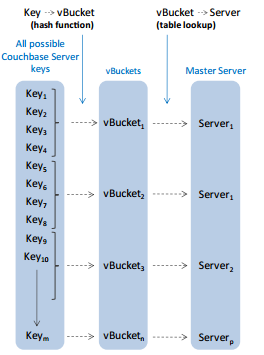
\includegraphics[width=0.4\textwidth]{img/vbucket2}
	\caption{ Couchbase Server vBucket ~\cite{couchbasedocs}}
	\label{fig:cb-vbucket}
\end{figure}
%where is reference of images

\paragraph{Data Model}%repeat check once
A document is a basic unit of data manipulation in Couchbase Server as a document store. All the documents are stored in JSON format without a predefined schema.

\paragraph{Querying and Indexing}
In Couchbase Server,  views are responsible for querying data from a bucket. Views are defined in a specific kind of document called \textit{design document}~\ref{fig:cb-views-design}. These documents are bounded to a single bucket and cannot be executed from other bucket. The design document holds JavaScript code that implements \textit{Mapreduce} operations to create view's index in user defined format. The Mapreduce is achieved by two functions \textit{map} and reduce. 
The \textit{map} function in design document identifies data from collection, process, filter them and output transformed values. Each document in a bucket is submitted to the \textit{map } function where document and metadata associated with the document are supplied as parameter to the \textit{map} function. After filtration, the \textit{emit} function in map returns the result as set of key/value pairs that are index. The output of map function can be zero or more "rows" according to the filter used in \textit{emit()} function. Each \textit{emit()} function returns a single row but can be called multiple times inside a single map function. The first parameter in \textit{emit} function is searchable text key and second parameter is the value.
The \textit{reduce} function is used to aggregate the numeric value generated in map phase. Couchbase has built-in reduce functions like \textit{\_count}, \textit{\_sum} and \textit{\_stats} aggregation. Table ~\ref{tbl:cb-mapreduce} illustrate an example of MapReduce  in Couchbase Server. The emit function at map phase returns the \textit{id} of document  as key and the price greater than 40 from documents that contains \textit{doctype} value "closed\_auctions". In \textit{reduce} phase, the the keys are grouped and values are counted.

%start here 

Query in Couchbase server has to be done against pre-materialize views as mentioned in section~\ref{intro-couchbase}. The goal of view is to select the data, extract the attributes and information as client's need  and to produce the index on selected information. In contrast to MongoDB,  couchbase's queries are closely associated with client SDK where each operations has to perform through SDKs. On-demand query language  named "N1QL" is also in  progress of development but still stable version has to be released~\cite{couchbasen1ql}.
%end here from benchmarking sections.
\begin{table}[H]
\begin{longtable}{c|c}
	\caption{Mapreduce in Couchbase Server}
	\label{tbl:cb-mapreduce}\\
	\textit{map()} & \textit{reduce()}\\
	\hline
\begin{minipage}{.6\textwidth}
\begin{fakeJSON}[label=cb-mapreduce-map,basicstyle=\small]
function (doc, meta) {
   if(doc.doctype && doc.doctype=="closed_auctions"){
     if(doc.price){
       if(doc.price > 40) {
	      emit(doc.id,doc.price)
     	}
    }
  }
}

\end{fakeJSON}	
\end{minipage} &
\begin{minipage}{.2\textwidth}
\begin{fakeJSON}[label=cb-mapreduce-reduce]
	_count
\end{fakeJSON}
\end{minipage}\\
\end{longtable}
\end{table}


\begin{figure}[H]
	\centering
	\subfloat[Views in Document Design]{
		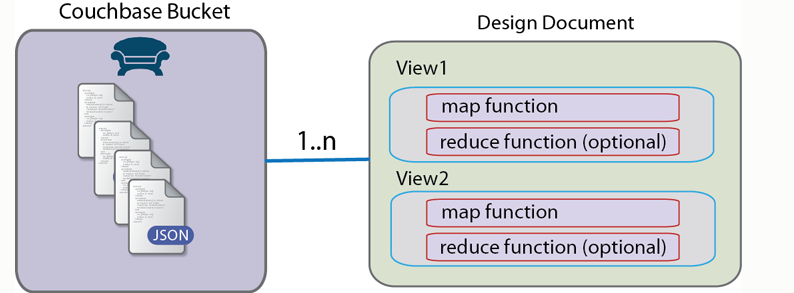
\includegraphics[width=0.4\textwidth]{img/cb/Small_view_elements}
		\label{fig:cb-views-design}
	}
	\centering
	\subfloat[View's Workflow]{
		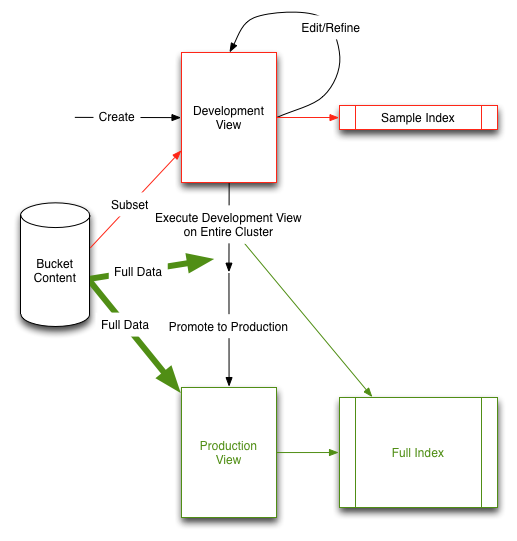
\includegraphics[width=0.4\textwidth]{img/cb/view-types-workflow}
		\label{fig:cb-views-workflow}
	}
	\caption{Couchbase Server's Document Design ~\citep{couchbasedocs}}
	\label{fig:cb-views-document-design}	
\end{figure}

	